\documentclass{article}
\usepackage{amsmath, amsfonts, amsthm, amssymb}
\usepackage{nips15submit_e,times}
\usepackage{hyperref} % for references within the document
\usepackage{url} % for URL links
\usepackage{graphicx} % for figures
\usepackage[round]{natbib}


\title{Recent Developments in Post-Selection Inference}


\author{
Yotam Hechtlinger\\
Department of Statistics\\
\texttt{yhechtli@andrew.cmu.edu} \\
\And
Shashank Singh \\
Department of Statistics \\
Machine Learning Department \\
\texttt{sss1@andrew.cmu.edu} \\
}

\newcommand{\fix}{\marginpar{FIX}}
\newcommand{\new}{\marginpar{NEW}}
\newcommand{\R}{\mathbb{R}}
\newcommand{\N}{\mathbb{N}}
\newcommand{\X}{\mathcal{X}}
\newcommand{\pr}{\mathbb{P}}
\newcommand{\E}{\mathbb{E}}
\newcommand{\sgn}{\operatorname{sign}}
\newcommand{\Unif}{\operatorname{Unif}}
\newcommand{\Nrm}{\mathcal{N}}
\newcommand{\poly}{\mathcal{P}}
\newcommand{\V}{\mathcal{V}}
\renewcommand{\hat}{\widehat}

\nipsfinalcopy % Uncomment for camera-ready version

\begin{document}
\maketitle

\begin{abstract}
It is common in modern applied statistics to use model selection tools, select
the most promising model, and then draw inference over the parameters of the
selected models. However, this simple series of actions conceals a significant
fault that is often left unattended: the act of selection biases the
distributions of test statistics and makes standard inference procedures
unsound. This is referred to as the problem of post-selection inference. We
review recent work that has shown how to correct for this in certain common
settings.
\end{abstract}

\section{Introduction}
In the linear regression setting, if $M$ denotes the set of indices for the
predictors spanning $X_M$, and $\hat\beta_M$ the least square
solution for the regression of $Y$ with $X_{M}$ predictors, then it is well
known that under the null hypothesis (i.e., the true coefficient is $0$), for
each $j \in M$,
\[Z_M^j
    := \frac{\hat\beta_M^j}{se\left(\hat\beta_M^j\right)}
    \sim \Nrm(0, 1),\]
This pivotal distribution is the driving force behind inference on least square
solutions. It is implicitly assumed that $\hat\beta_M^j$ was chosen to be the
predictor of interest prior to sampling the data, and hence the model is fixed.
Furthermore, it is also assumed that the only predictor of interest is $j$,
thought, there is a need to provide inference over a larger set of predictors,
standard corrections for multiple comparisons, such as the Bonferonni
correction, can be used.

In practice, the widespread use of model selection tools introduces a
stochastic component to selection of the model. When the data is being used
twice (i.e., for both model selection and inference), the assumption of a fixed
model is violated and the inference is no longer sound.

\subsection{An illustrative simulation}
The following simulation demonstrates the problem in a simple case, which,
unfortunately, can describe an enthusiastic but naive researcher hunting for a
discovery. Consider $p$ independent predictors,
$X_1,\ldots,X_p \sim \Nrm(0, 1)$ and an independent observation vector
$Y\sim\mathcal{N}\left(0,1\right)$ (i.e., all vectors are independent random
noise). In order to find the most promising predictor explaining $Y$, $p$
different univariate regression models are fitted to $Y$, and the most
significant is chosen at each iteration. Figure \ref{fig:sim} shows the
distribution of $\max_{j,M} Z_M^j$ as a function of the number of predictors
$p$. 

In the simulation, univariate regression was done in order to simplify
the example. In multivariate model selection, a model $X_M$ has
$|M|$ different predictors. Although there is dependence
between the statistics of the same predictor between different models,
naively correcting for the maximum would require
$\sum_{k = 1}^p \binom{p}{k} k$ tests. This exponential growth results in
performing $192$ different tests for $p = 6$, emphasizing that the unsound
distribution of $n = 100$, presented in Figure $1$, offering less than $8\%$
coverage, is easily accessible with improper use of model selection, even in
low-dimensional settings.

\begin{figure}
\begin{center}
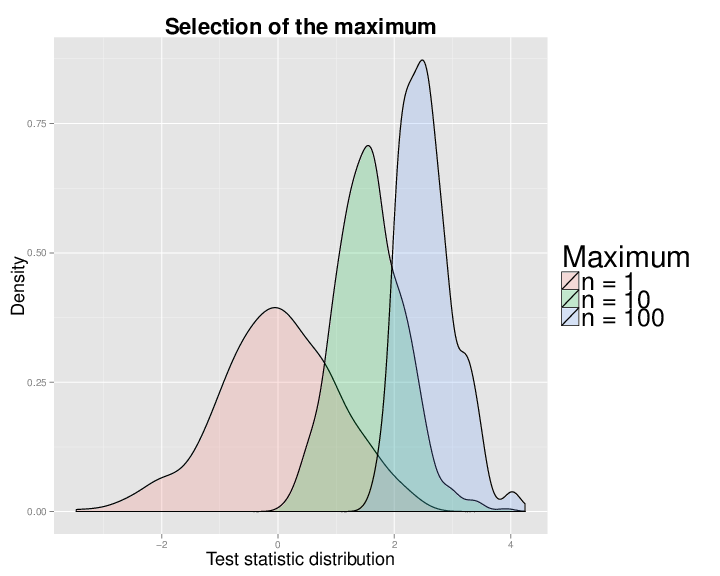
\includegraphics[width=0.7\textwidth]{figures/Maxdist}
\end{center}
\caption{The distribution of $\max_{j,M} Z_M^j$, for several values of the
dimension, $p$. When $p = 1$, $Z_M^j \sim \Nrm(0, 1)$. However, as $p$
increases, rejecting at $|Z_M^j| > z_{\alpha/2}$ is almost certain to provide
false positive results.}
\label{fig:sim}
\end{figure}

\subsection{Historical approaches to the post-selection inference problem}
One approach to ensuring validity of post-selection inference technically
embeds the problem in the field of multiple comparisons. By approaching each
coefficient inference as a single inference, controlling the family-wise error
rate over the family of inferences guarantees valid inference for the selected
model. The simplest such solution is to apply a Bonferroni correction,
dividing the type I error threshold by the (large) number of tests being
performed.
Recently, \citet{berk13PoSI} provided a less conservative approach
which simultaneously bounded all linear functions that arise as coefficient 
estimates in all submodels.
However, due to the exponential growth of the number of inferences
as a function of dimension, these simultaneous methods quickly become too
conservative.

A more precise solution to the problem requires accounting for the specific
nature of the selection procedure. For the example above, this is quite
straightforward; since each $Z_M^j \sim \Nrm(0, 1)$, $\max_{_M,j} Z_M^j$ has
the cumulative distribution function (CDF) $\Phi^p$, where $\Phi$ denotes the
CDF of $\Nrm(0, 1)$, and, therefore,
\[\mathbb{P}_{H_{0}}\left(\max_{j,M} Z_M^j \in [-c,c] \right)
    = \Phi^{p}\left(c\right)-\Phi^{p}\left(-c\right).\]


For $p \geq 3$, $\Phi^{p}\left(-c\right) \approx 0$, and a one sided test
typically suffices. Thus a valid acceptance region controls
$\Phi^p\left(c\right) = 1 - \alpha$, which is equivalent to rejecting when
$c \geq z_{\left(1-\alpha\right)^{1/p}}$.

In more general cases, understanding the distribution of the statistics
conditioned on the selection is not as trivial. Conditional inference has been
actively researched throughout the years by
\citet{buehler63students,brown67students,olshen73fTest}, and others.
\citet{weinstein13morePower} provide a conditional approach towards confidence
intervals for the case of Gaussian distributions, which can be utilized when
selection is determined by some predefined threshold (say $z_{1-\alpha/2}$).

\subsection{Recent progress}
In this project we cover two recent breakthroughs in the conditional inference
school, which have contributed substantially to solving the problem of
post-selection inference in several settings.

The first is a paper by \citet{fithian14optimal}, approaches conditional
inference in general way, defining conditional tests and confidence intervals,
and then demonstrating how to do conditional inference in the exponential
family setting. This results in important conceptual tools that are not always
easy to compute from real data.

The second paper, due to \citet{taylor14post}, considers the special case of a
Gaussian noise model and a specific class of \emph{polyhedral} selection
procedures which select variables based on a set of affine constraints on the
response variable. In this case, they are able do derive $p$-values and
selection intervals for exact inference conditioned on the model selected.
While this approach has less generality, in contrast to
\citet{fithian14optimal}, \citet{taylor14post} are able to give easily
computable tools for inference, as well as strong, computationally efficient
approximations for several common selection procedures.

In the following sections we will present the methods and results of both
\citet{fithian14optimal} and \citet{taylor14post} in greater detail, and then
conclude with a general discussion of post-selection inference.

\section{Conditioning on selection in exponential families}
\label{sec:fithian}

\citet{fithian14optimal} provide general definitions and notation towards
conditional inference, and demonstrate how it can be performed in an
exponential family setting. Their leading guideline for inference is that it
``\textit{must be valid, given that the question was asked}'', where question
is precisely defined as a tuple $\left(M,H_{0,j}^M \right)$, testing the
hypothesis $H_{0,j}^{M}$ for the $j$ predictor in the selected model $M$. In
that case, a level-$\alpha$ selective test is expected to control the selective
type I error:

\[\mathbb{P}_{M,H_0}\left(\text{reject}H_{0,j}^M
                | \left(M,H_{0,j}^M\right)\text{ selected}\right)
                                                                \leq \alpha.\]

But in their paper, \cite{fithian14optimal}, develop an even more general
framework for the problem. For any event $A$, hypothesis test will
be a function $\phi\left(y\right)$ of the random variable $Y$, taking
values in $\left[0,1\right]$, and is said to controls the selective
type I error if

\[
\mathbb{E}_{F}\left[\phi\left(Y\right)\mid A\right]\leq\alpha,\;\text{for all
}F\in H_{0}.
\]

Adopting the conditional point of view, classical statistical theory
can be restated in a conditional manner, defining selective power
function, selective confidence intervals, selective unbiased test and
inadmissibility as expected. For example, selective confidence intervals
would have $1-\alpha$ coverage for the parameter $\theta\left(F\right)$
if

\[
\mathbb{P}_{F}\left(\theta\left(F\right)\in C\left(Y\right)\mid
A\right)\geq1-\alpha,\;\text{for all }F\in H_{0},
\]
and this can be obtained by inverting selective tests, as in the classical
case. 

The major problem remaining is how to control the distribution of
the statistics in a conditional manner. The general case is often
quite hard, but the main result of the paper demonstrates that for
test statistics with exponential family distributions it follows naturally. 

If $Y$ follows a multi-parameter exponential family, than by the
factorization theorem

\[
Y\sim\exp\left\{ \theta^{'}T\left(y\right)-\psi\left(\theta\right)\right\}
f_{0}\left(y\right),
\]
and in that case, conditioning $Y$ on the event $A$, will be equivalent
to

\[
\left(Y\mid Y\in A\right)\sim\exp\left\{
\theta^{'}T\left(y\right)-\psi\left(\theta\right)\right\}
f_{0}\left(y\right)\mathbb{I}\left\{ y\in A\right\} ,
\]
which by the factorization theorem also represent exponential family.
This reduces the problem to a well known problem of exponential family
inference, in which many classical tools are available, one in specific
is the uniformly most powerful unbiased (UMPU) test developed by
\cite{lehmann55estimation}. 

But even with the UMPU test, in order to compute the test values,
it is required to know the likelihood function,
$\mathcal{L}_{\theta}\left(Y\mid A\right)$,
for all $\theta\in\Theta$. In simple cases this can be computed explicitly,
such as the selection of the maximum described in the simulation.
In most cases of selection, Monte Carlo methods are required for the
exact calculation.

The final point to be discussed is the decision on which event $A$
to perform the conditioning. $A$ must be generated from a selection variable 
partitioning the space for the different models, but there are many ways to 
partition the space in such a way, and the inference can vary significantly by
the selection of the conditioning event. An important result demonstrates that 
the finer the partition of the selection variable, the more information to be 
gained by conditioning.

A specific case would be data splitting, which can be considered as a scenario
in which conditioning discards all the information on the training set. A finer
partition would condition on the value observed by the training set resulting
in the model selected. The paper demonstrates that it will almost always be
possible to choose a finer partition than the one used for data splitting that
would always yield more power, and hence data splitting is inadmissible. 

\section{The special case of Gaussian inference after polyhedral selection}
\label{sec:taylor}
\citet{taylor14post} pioneer a new exact approach to post-selection inference
for a class of variable selection procedures that are \emph{polyhedral} (as
defined in Section \ref{subsec:poly}). For such selectors, they derive
exact $p$-values for testing the significance of predictor variables,
conditioned on the results of variables selection.

To do this, they make two assumptions on the distributions of the true data.
First, they assume the covariate matrix $X$ lies in general position (a very
weak rank-like assumption, which is satisfied almost surely by continuously
distributed variables). The second and more restrictive assumption is that the
noise is Gaussian. That is, the true model has the form
\begin{equation}
y = \theta(x) + \varepsilon,
\label{eq:Gauss_model}
\end{equation}
where $\varepsilon \sim \mathcal{N}(0,\Sigma)$ and $\theta : \R^p \to \R$ is
some (not necessarily linear) function of the predictors.

In this section, we first describe the structure of polyhedral selection, and
outline how this allows us to perform valid post-selection inference under
the model (\ref{eq:Gauss_model}). We then show that several common variable
selection procedures are polyhedral, and derive the corresponding
post-selection inference procedures.

\subsection{Polyhedral selection}
\label{subsec:poly}
Suppose we observe $n$ samples of $p$ predictor variables
$(x_1,\dots,x_p) \in \R^p$ and a corresponding response variable $y \in \R$,
giving a covariate matrix $X \in \R^{n \times p}$ and a response vector
$y \in \R^n$.

Recall that a polyhedron in $\R^n$ is any set $\poly \subseteq \R^n$ defined by
a finite set of affine constraints (i.e.,
$\poly = \{z \in \R^n : \Gamma z \geq u\}$ for some
$\Gamma \in \R^{m \times n}, u \in \R^m$, where the inequality holds
component-wise). A variable selection procedure is called \emph{polyhedral} if,
for any covariate matrix $X \in \R^{n \times p}$, the sets of outcomes
$y \in \R^n$ resulting in any particular selection of variables with particular
correlation signs $\sgn(X_j^T y)$ are all polyhedra.

\begin{figure}[ht]
\begin{center}
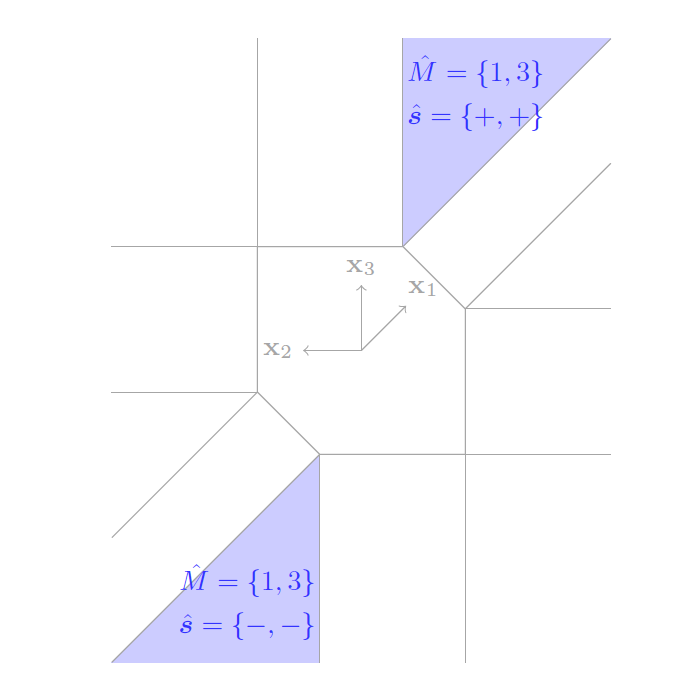
\includegraphics[width=0.5\textwidth]{figures/polyhedral}
\end{center}
\vspace{-5mm}
\caption{Illustration of marginal screening as a polyhedral selector.
Here, we observe two samples and have three covariates. If the response
$y \in \R^2$ falls in either shaded region, then variables $x_1$ and $x_3$ will
be selected (as they are sufficiently correlated with $y$, while $x_2$ is not).
The bottom left and top right regions corresponds to negative and positive
correlations, and hence negative and positive estimated coefficients,
respectively.}
\label{fig:polyhedral}
\end{figure}

As an illustrative example, a very simple polyhedral selection procedure is
\emph{marginal screening} (MS), illustrated in Figure \ref{fig:polyhedral}. MS
simply selects those variables which are sufficiently correlated with the
response. That is, for some $c \in [0,1]$, MS will select a variable $x_j$ if
and only if $|X_j^Ty| \geq c\|X_j\|_2$, where $c$ can be chosen based on
desired number of selected variables.

Suppose for instance, that MS selects the
$\ell$ variables $\{x_{k_i}\}_{i = 1}^\ell$ with a particular sequence
$\{s_i\}_{i = 1}^\ell = \{\sgn(X_{k_i}^T y)\}_{i = 1}^\ell$ of signs. This
occurs if and only if, for each selected $x_{k_i}$,
$X_{k_i}^T y \geq c\|X_{k_i}\|_2$ and, for each unselected $x_j$,
both $X_j^Ty \leq c\|X_j\|_2$ and $-X_j^Ty \leq c\|X_j\|_2$. Thus, if, for each
$i \in \{1,\dots,\ell\}$, $\Gamma \in \R^{(k + 2(p - k)) \times n}$ has a row
$s_i X_{k_i}^T$ and $u \in \R^n$ has a corresponding entry $c\|X_{k_i}\|_2$,
and for each $j \notin \{k_1,\dots,k_\ell\}$, $\Gamma$ has two rows, $X_j^T$
and $-X_j^T$, and $u$ has two corresponding entries, both $-c\|X_j\|_2$.
See \citet{lee14marginalScreening} for a detailed study of inference after
model selection through marginal screening.

The next section presents two lemmas, which together suggest how to perform
exact post-selection inference after polyhedral selection.

\subsection{Conditional Gaussian inference after polyhedral selection}
\label{subsubsec:lemmas}

The hypothesis that $y$ is uncorrelated with $x_j$ can be phrased as
$x_j^T \theta = 0$ (recalling that $y$ is $\theta$ plus noise), suggesting that
we are interested in the distribution of $v^T y$ for certain $v \in \R^n$. The
lemma 1 gives an representation of a polygon in terms of terms of arbitrary
such $v \in \R^n$.

\begin{figure}[ht]
\begin{center}
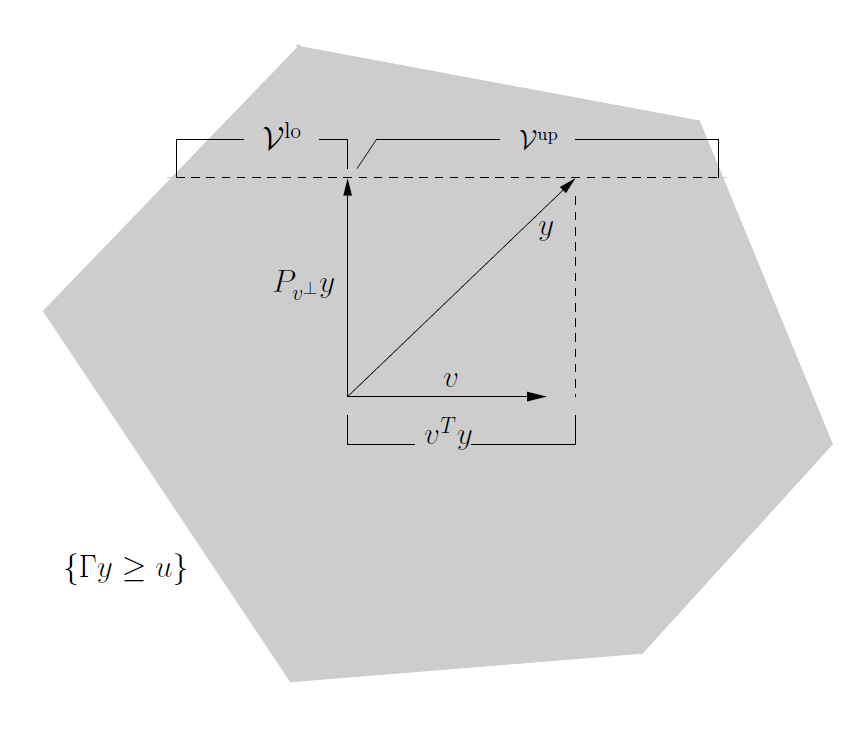
\includegraphics[width=0.5\textwidth]{figures/polyhedral_testing}
\end{center}
\vspace{-5mm}
\caption{Illustration of the polyhedron
$\poly = \{y \in \R^n : \Gamma y \geq u\}$ encoded in terms of $\V^{lo}(y)$,
$\V^{hi}(y)$, and $\V^0(y)$. Since $v$ points precisely to the right
$\V^{lo}(y)$ encodes the rightmost constraint to the left of $y$, $\V^{hi}(y)$
encodes the leftmost constraint to the right of $y$, and $\V^0(y)$ encodes
constraints parallel to $v$ (of which none are shown here).}
\label{fig:encoded_poly}
\end{figure}

{\bf Lemma 1 (Polyhedral selection as truncation):}
Suppose $y \sim \mathcal{N}(\theta,\Sigma)$, where $\theta \in \R^n$ is unknown
but $\Sigma \in \R^{n \times n}$ is known. Consider a polyhedron
$\poly = \{y \in \R^n : \Gamma y \geq u \}$, where $\Gamma \in \R^{m \times n}$
and $u \in \R^m$. If $v^T \Sigma v \neq 0$, then, for
\[\rho := \frac{\Gamma \Sigma v}{v^T \Sigma v},
    \quad \V^0(y) := \max_{j : \rho_j = 0} u_j - (\Gamma y)_j,\]
\[\V^{hi}(y) := \min_{j : \rho_j > 0}
    \frac{u_j - (\Gamma y)_j + \rho_j v^T y}{\rho_j},
    \quad \mbox{ and } \quad
\V^{lo}(y) := \max_{j : \rho_j < 0}
    \frac{u_j - (\Gamma y)_j + \rho_j v^T y}{\rho_j},\]
$(\V^0(y),\V^{hi}(y),\V^{lo}(y))$ is independent of $v^T y$ and
\[y \in \poly
    \quad \Leftrightarrow \quad
    \V^0(y) \leq 0
    \mbox{ and }
    v^T y \in [\V^{lo}(y), \V^{hi}(y)].\]

The intuition behind Lemma 1 is illustrated in Figure \ref{fig:encoded_poly}.
The independence results from the fact that $(\V^0(y),\V^{hi}(y),\V^{lo}(y))$
is a function of $y - \frac{\Sigma v v^T y}{v^T \Sigma v}$, which is
independent of $v^T y$ because $y \sim \Nrm(\theta,\Sigma)$.

Since $v^T y$ has a Gaussian distribution, Lemma 1 tells us that
$v^T y | y \in \poly$ has a $1$-dimensional truncated Gaussian distribution.
We now establish some notation which will allow us to construct our desired
test statistic.

For $a,b,\mu,\sigma \in \R$ with $a < b$, $\sigma > 0$, let
$F_{\mu,\sigma^2}^{[a,b]}$ denote the CDF of $\Nrm(\mu, \sigma^2)$ truncated
to $[a,b]$, i.e.,
\[F_{\mu,\sigma^2}^{a,b}(x)
    = \frac{\Phi\left( \frac{x - \mu}{\sigma} \right)
                                - \Phi\left( \frac{a - \mu}{\sigma} \right)}
    {\Phi\left( \frac{b - \mu}{\sigma} \right)
                                - \Phi\left( \frac{a - \mu}{\sigma} \right)},
    \quad \forall x \in [a,b].
\]
where $\Phi : \R \to \R^+$ denotes the CDF of $\Nrm(0, 1)$.
We then have the following pivotal statistic: \\

{\bf Lemma 2 (Conditional $p$-values):} For $v \in \R^n$,
$\Sigma \in \R^{n \times n}$, if $v^T \Sigma v \neq 0$, then
\[F^{\V^{lo}(y), \V^{hi}(y)}_{v^T \theta, v^T \Sigma v}(v^T y) | y \in \poly
    \sim \Unif(0,1),\]
i.e., $F^{\V^{lo}(y), \V^{hi}(y)}_{v^T \theta, v^T \Sigma v}(v^T y)$ is a valid
$p$-value conditioned on $y \in \poly$.

The proof of Lemma 2 is also fairly simple, and depends essentially on the
independence of $(\V^0,\V^{lo},\V^{hi})$ and $v^T y$. Lemma 2 in turn gives
rise to the following two-sided conditional hypothesis test (testing
$H_0 v^T \theta = 0$ against $H_1 : v^T \theta \neq 0$):
\footnote{A more powerful one-sided conditional test for the alternative
$H_1 : v^T \theta > 0$ is similarly easy to derive.} \\

{\bf Lemma 3 (Two-sided conditional inference after polyhedral selection):}
Suppose $v^T \Sigma v \neq 0$. Define the statistic
\[T := 2 \min \left\{ F^{\V^{lo}(y),\V^{hi}(y)}_{0,v^T \Sigma v}(v^T y),
            1 - F^{\V^{lo}(y),\V^{hi}(y)}_{0,v^T \Sigma v}(v^T y) \right\}.\]
Then, $T$ is a valid conditional $p$-value for $H_0$; i.e., under $H_0$,
$T | y \in \poly \sim \Unif(0,1)$. \\

\subsection{Application to forward stepwise regression}
In section \ref{subsec:poly}, we showed that a simple selection procedure,
marginal screening, is polyhedral. A somewhat more elaborate selection
procedure, forward stepwise regression (FS), is discussed by
\citet{taylor14post}.

FS is an iterative procedure, which, in each iteration, adds the variable
causing the largest drop in residual error.
\footnote{The assumption that $X$ has columns in general position guarantees
uniqueness of the selected variables and their signs.}
In particular, let $A_k = [j_1,\dots,j_k]$ and $s_{A_k} = [s_1,\dots,s_k]$
denote the ordered list of active variables and their signs (upon entering)
after $k$ iterations. Since FS greedily chooses variables which minimize the
residual sum of squares (RSS), for any $j \notin \{j_1,\dots,j_k\}$,
\begin{equation}
RSS(y,X_{A_k}) \leq RSS(y,X_{A_{k - 1} \cup \{j\}})
\label{ineq:FS_RSS}
\end{equation}
and
\begin{equation}
s_k = \sgn(e_k^T (X_{A_k})^+ y).
\label{eq:FS_sign}
\end{equation}
This allows us to express FS as a polyhedral selection method, as follows.

{\bf Theorem 1 (FS selection is polyhedral):} The set
\[\poly := \{y \in \R^n : \hat A_k(y) = A_k, \hat s_{A_k}(y) = s_{A_k}\}\]
of response vectors $y$ resulting in the FS active set $A_k$ and signs
$s_{A_k}$ is a polyhedron $\poly = \{y \in \R^n : \Gamma y \geq 0\}$. \\

\emph{Proof:}
We construct $\Gamma$ iteratively by adding $2(p - k)$ rows in the $k^{th}$
iteration, corresponding to the $k^{th}$ iteration of FS. If $j_k$ and $s_k$
are the first variable and sign chosen by FS, then the conditions
(\ref{ineq:FS_RSS}) and (\ref{eq:FS_sign}) are equivalent to
\[\frac{s_1X_{j_1}^T}{\|X_{j_1}\|_2} \geq \pm \frac{X_j^Ty}{\|X_j\|_2},
    \quad \forall j \notin A_k.\]
Thus, we add to $2(p - k)$ rows to $\Gamma$, of the form
\[\frac{s_1X_{j_k}^T}{\|X_{j_1}\|_2} \pm \frac{X_j}{\|X)j\|_2},\]
(with one row for each pair of $\pm$ and $j \notin A_k$). \qed

To test the null hypothesis $H_0 : v^T \theta = 0$ against
$H_1 : v^t \theta \neq 0$, we simply compute $\V^{lo}(y),\V^{hi}(y),\V^0(y)$ as
in Lemma 1 and then use the test statistic
\[T_k := 2\min\left\{ F^{[\V^{lo}(y),\V^{hi}(y)]}_{0,\sigma^2\|v\|_2^2}(v^T y),
        1 - F^{[\V^{lo}(y),\V^{hi}(y)]}_{0,\sigma^2\|v\|_2^2}(v^T y)\right\},\]
and, similarly, a $(1 - \alpha)$-confidence intervals for $v^T \theta$ is
$[\delta_{\alpha/2}, \delta_{1 - \alpha/2}]$ satisfying
\[1 - F^{[\V^{lo}(y),\V^{hi}(y)]}_{\delta_{\alpha/2},\sigma^2\|v\|_2^2}(v^T y)
    = \alpha/2\]
and
\[1 - F^{[\V^{lo}(y),\V^{hi}(y)]}
                    _{1 - \delta_{\alpha/2},\sigma^2\|v\|_2^2}(v^T y)
    = 1 - \alpha/2.\]

\subsection{Other consequences}
The ideas presented in Section \ref{subsubsec:lemmas} can be applied and
extended in a straightforward manner to derive other useful tools for model
selection and post-selection inference, some of which we discuss below.

{\bf Other Selection Procedures:} \citet{lee13lasso} apply the polyhedral
selection framework for the lasso at any value of the regularization parameter
$\lambda$ and derive appropriate $p$-values and selection intervals.
\citet{taylor14post} do the same for least angle regression (LAR). Because, in
practice the $\Gamma$ constraint matrix used in Lemma 1, can grow very large
(with roughly $4pk$ rows after $k$ steps of LAR), \citet{taylor14post} also
derive an much smaller approximate set of constraints (with at most $k + 1$
rows), which they show yields a highly accurate and computationally efficient
approximation to the true selection polyhedron.

{\bf Selection Intervals:} The hypothesis test presented in Lemma 3 can be
inverted to compute exact selection intervals (as described in Section
\ref{subsec:select_ints}).

{\bf Stopping Rules:} Using general methods for sequential hypothesis testing
from \citet{gsell13sequentialSelection}, we can establish a stopping rule for
iterative selection methods (such as FS and LAR) with guarantees on the false
discovery rate.

\section{Discussion}
\subsection{Coverage in Model Selection}
\label{subsec:coverage}
It is important to emphasize that the entire field of inference after model
selection is highly susceptible to the assumptions. Without the (usually
unreasonable) assumption that the true model is generated by the linear model
just selected, the meaning of the coefficients is vague. Even assuming that
there exists a real coefficient vector $\beta$ generating $Y$ in a linear way,
any selected model will typically contain a subset of $\beta$, in which each of
the selected components is a linear combination of the full vector $\beta$. In
particular, any estimator upon which we perform inference is highly influenced
by correlations with predictors that are not selected. This point has been
demonstrated in and studied in depth by \citet{gsell13false}.
One way of defining coverage in this context is as in \citet{berk13PoSI}, in
which an estimator should reliably cover its own expected value. This addresses
the problem of defining confidence intervals and valid tests, although the
interpretation of the interval is still unclear, as the expected value is also
affected by the unselected predictors.

\subsection{Selection Intervals}
\label{subsec:select_ints}
As mentioned previously, conditional hypothesis test such as that presented in
Lemma 3 can be inverted to compute \emph{selection intervals}. In contrast with
traditional confidence intervals, selection intervals guarantee coverage of the
expectation of a parameter (which is itself a random variable resulting from
model selection), consistent with the notion of conditional inference given in
Section \ref{subsec:coverage}. That is, we can find an interval $I$ around an
estimated coefficient $\hat\beta_j$ with the property
\[\pr\left[ \E[\hat\beta_j] \in I | y \in \poly \right] = 1 - \alpha.\]

\subsection{Unconditional Inference}
\citet{taylor14post} point out a simple but important observation that
characterizes the utility of conditional hypothesis tests. In particular, if
$A$ is the event of a type 1 error, then, for a valid $\alpha$-level hypothesis
test conditioned on some random variable $X = x$,
\[\alpha \geq \pr\left[ A | X = x \right]
    = \frac{\pr\left[ A,X = x \right]}{\pr\left[ X = x \right]}
    \geq \pr\left[ A,X = x \right].\]
Then, integrating over $x$ gives $\alpha \geq \pr\left[ A \right]$. Thus, a
valid conditional $\alpha$-level hypothesis test is also a valid unconditional
$\alpha$-level hypothesis test. In the case of variable selection, $X$ might be
the subset of selected variables. In fact, a similar argument shows that the
conditional hypothesis is valid for any coarsening of the condition; for
example, a valid test conditioned on $X = x$ would also be a valid test
conditioned on $X \subseteq \X$, for any set $\X$ containing $x$.

\section{Conclusion}
We reviewed the general problem of post-selection inference, as well as two
recent lines of work which attempt to solve the problem in certain special
cases.

\small{
\bibliographystyle{plainnat}
\bibliography{biblio}
}

\end{document}
